%%%%%%%%%%%%%%%%%%%%%%%%%%%%%%%%%%%%%%%%%%%%
% FILE KONFIGURASI TEMPLATE LATEX
%%%%%%%%%%%%%%%%%%%%%%%%%%%%%%%%%%%%%%%%%%%%

\usepackage[american]{babel}
\usepackage[utf8]{inputenc}
\usepackage{geometry}
\geometry{
	a4paper,
	left=40mm,
	top=35mm,
	right=30mm,
	bottom=30mm
}

% --- Paket Dasar & Algoritma ---
\usepackage{algorithm}
\usepackage{algpseudocode}
\renewcommand{\algorithmicrequire}{\textbf{Input:}}
\renewcommand{\algorithmicensure}{\textbf{Output:}}

% --- Paket Tampilan & Grafik ---
\usepackage{graphicx}
\usepackage{epsfig}
\usepackage{subcaption}
\usepackage{pdflscape}
\usepackage{lscape}
\usepackage{rotating}
\usepackage{adjustbox}
\usepackage{wrapfig}
\usepackage{float}
\usepackage{morefloats}
\usepackage{eso-pic}
\usepackage{pdfpages}

% --- Background Image ---
\newcommand\BackgroundIm{
	\put(0,0){
		\parbox[b][\paperheight]{\paperwidth}{%
			\vfill
			\centering
			\includegraphics[height=\paperheight,keepaspectratio]{./lib/background.png}%
			\vfill
}}}

% --- Paket Tabel ---
\usepackage{booktabs}
\setlength{\heavyrulewidth}{\lightrulewidth}
\usepackage{longtable}
\usepackage{multirow}
\usepackage{array,tabularx}
\usepackage[table,xcdraw]{xcolor}

% --- Paket Matematika & Simbol ---
\usepackage[fleqn]{amsmath}
\usepackage{amsfonts}
\usepackage{amssymb}
\usepackage{nccmath}
\usepackage{pifont}

\newcommand{\cmark}{\checkmark}
\newcommand{\xmark}{\ding{55}}
\newcommand{\specialcell}[1]{\begin{tabular}[c]{@{}c@{}}#1\end{tabular}}

% --- Paket Teks & Format ---
\usepackage{setspace}
\setstretch{1.5}
\linespread{1.5}
\usepackage{type1cm}
\usepackage{lettrine}
\usepackage{enumitem}
\usepackage{ulem}
\usepackage{titlesec}
\usepackage{multicol}
\usepackage{listings}
\usepackage{ragged2e}
\usepackage{lipsum}
\usepackage{hyphenat}
\usepackage{comment}
\usepackage{changepage}
\usepackage{afterpage}

% --- Referensi & Sitasi ---
\usepackage[round,authoryear]{natbib}
\usepackage{hyperref}
\hypersetup{hidelinks}
\usepackage[pageref]{backref}
\usepackage[nameinlink]{cleveref}

% --- Pengaturan Header & Footer ---
\usepackage{fancyhdr}
\usepackage{etoolbox}
\usepackage{url}
\usepackage{makeidx}
\makeindex

\fancyhf{}
\renewcommand{\headrulewidth}{0pt}
\pagestyle{fancy}
\fancyfoot[CE,CO]{\thepage}
\patchcmd{\chapter}{empty}{plain}{}{}

% --- Lingkungan / Environment Khusus ---
\newenvironment{FontCover}{\fontfamily{phv}\selectfont}{\par}

\newenvironment{Kondisi}
{\par\vspace{\abovedisplayskip}\noindent
	\tabularx{\columnwidth}{>{$}l<{$} @{${}:{}$} >{\raggedright\arraybackslash}X}}
{\endtabularx\par\vspace{\belowdisplayskip}}

\newenvironment{conditions}
{\par\vspace{\abovedisplayskip}\noindent
	\tabularx{\columnwidth}{>{$}l<{$} @{${}={}$} >{\raggedright\arraybackslash}X}}
{\endtabularx\par\vspace{\belowdisplayskip}}

% Fix titlesec bug
\makeatletter
\patchcmd{\ttlh@hang}{\parindent\z@}{\parindent\z@\leavevmode}{}{}
\patchcmd{\ttlh@hang}{\noindent}{}{}{}
\makeatother

% --- Pengaturan Section & Judul ---
\titleformat{\chapter}[display]{\bfseries\Large}{CHAPTER \centering\thechapter}{0ex}{\vspace{0ex}\centering}[\vspace{3ex}]
\titlespacing*{\chapter}{0pt}{-4ex}{0pt}
\titleformat{\section}{\bfseries\normalsize}{\MakeUppercase{\thesection}}{1ex}{}
\titleformat{\subsection}{\normalsize\bfseries}
\titleformat{\subsubsection}{\normalsize\bfseries}

\titlespacing{\section}{0pt}{0pt}{1ex}
\titlespacing{\subsection}{0pt}{0pt}{1ex}
\titlespacing{\subsubsection}{0pt}{0pt}{1ex}

% --- Caption Setup ---
\usepackage[labelfont=bf]{caption}
\captionsetup{labelfont=bf}
\captionsetup[figure]{font=small,skip=15pt}
\captionsetup[table]{font=small,skip=15pt}

\setlength{\floatsep}{8pt plus 2pt minus 2pt}
\setlength{\textfloatsep}{10pt plus 2pt minus 2pt}
\setlength{\intextsep}{10pt plus 2pt minus 2pt}

\DeclareCaptionLabelSeparator{none}{}
\captionsetup{labelsep=period}
\renewcommand{\figurename}{Figure}
\renewcommand{\tablename}{Table}
\renewcommand{\lstlistingname}{Code}

\setcounter{secnumdepth}{5}
\hyphenation{meng-gerak-kan mem-per-kenal-kan pe-ri-la-ku di-je-las-kan mem-bu-tuh-kan me-ne-rap-kan}

\def\kosong{
	\vspace*{\fill}
	\begin{center}\textit{This page is intentionally left blank}\end{center}
	\vfill
}
\patchcmd{\cleardoublepage}{\hbox{}}{\kosong}{}{}

\renewcommand*{\backreflastsep}{, }
\renewcommand*{\backreftwosep}{, }
\renewcommand*{\backref}[1]{}

% --- Bolean Variables ---
\newboolean{PembimbingDua}
\setboolean{PembimbingDua}{false}

\newboolean{bThesis}
\setboolean{bThesis}{true}

\newboolean{PembimbingTiga}
\setboolean{PembimbingTiga}{false}

\newboolean{PembimbingInternasional}
\setboolean{PembimbingInternasional}{false}

\newboolean{PengujiTiga}
\setboolean{PengujiTiga}{false}

\newboolean{PengujiEmpat}
\setboolean{PengujiEmpat}{false}

\newboolean{Nomenklatur}
\setboolean{Nomenklatur}{false}

\newboolean{bDoktor}
\setboolean{bDoktor}{false}

\newboolean{bMaster}
\setboolean{bMaster}{false}

\newboolean{JudulTesisEng}
\setboolean{JudulTesisEng}{false}

\renewcommand{\em}[1]{\textit{#1}}
\renewcommand{\emph}[1]{\textit{#1}}

% --- Definisi Perintah Identitas & Penguji ---
\newcommand{\Mahasiswa}[2]{
	\newcommand{\NamaMahasiswa}{#1}
	\newcommand{\NrpMahasiswa}{#2}
}

\newcommand{\PembimbingSatu}[2]{
	\newcommand{\PbSatu}{#1}
	\newcommand{\NipPbSatu}{#2}
}

\newcommand{\PembimbingDua}[2]{
	\setboolean{PembimbingDua}{true}
	\newcommand{\PbDua}{#1}
	\newcommand{\NipPbDua}{#2}
}

\newcommand{\PembimbingTiga}[2]{
	\setboolean{PembimbingTiga}{true}
	\newcommand{\PbTiga}{#1}
	\newcommand{\NipPbTiga}{#2}
}

\newcommand{\PengujiSatu}[2]{
	\newcommand{\PjSatu}{#1}
	\newcommand{\NipPjSatu}{#2}
}

\newcommand{\PengujiDua}[2]{
	\newcommand{\PjDua}{#1}
	\newcommand{\NipPjDua}{#2}
}

% FIXED: Menyesuaikan pembuatan variabel Penguji Tiga
\newcommand{\PengujiTiga}[2]{
	\setboolean{PengujiTiga}{true}
	\newcommand{\PjTiga}{#1}
	\newcommand{\NipPjTiga}{#2}
}

% FIXED: Mengaktifkan dan melengkapi variabel Penguji Empat
\newcommand{\PengujiEmpat}[2]{
	\setboolean{PengujiEmpat}{true}
	\newcommand{\PjEmpat}{#1}
	\newcommand{\NipPjEmpat}{#2}
}

\newcommand{\KaDep}[2]{
	\newcommand{\NmKaDep}{#1}
	\newcommand{\NipKaDep}{#2}
}

\newcommand{\CoverFooter}[1]{\newcommand{\bdk}{#1}}
\newcommand{\Judul}[1]{\newcommand{\JdTesis}{#1}}
\newcommand{\TanggalUjian}[1]{\newcommand{\TglUjian}{#1}}
\newcommand{\PeriodeWisuda}[1]{\newcommand{\PerWisuda}{#1}}
\newcommand{\Fakultas}[1]{\newcommand{\fak}{#1}}
\newcommand{\BeltFakultas}[1]{\newcommand{\bbelt}{#1}}
\newcommand{\Departemen}[1]{\newcommand{\Dep}{#1}}

\newcommand{\ggGelar}{xxxx}
\newcommand{\pPengesahan}{xxxxxxxx}

\newcommand{\Gelar}[1]{\renewcommand{\ggGelar}{#1}}
\newcommand{\tsss}{This dissertation is prepared to fulfill the requirements for obtaining\\the degree of}

\newcommand{\Disertasi}[1]{
	\renewcommand{\tsss}{This dissertation is prepared to fulfill the requirements for obtaining\\the degree of}
	\renewcommand{\pPengesahan}{STATEMENT OF APPROVAL}
	\renewcommand{\ggGelar}{#1}
	\setboolean{bMaster}{false}
	\setboolean{bThesis}{true}
}

\newcommand{\prop}{PROPOSAL DISERTASI}
\newcommand{\ProposalDisertasi}{
	\renewcommand{\prop}{PROPOSAL DISERTASI}
	\setboolean{bMaster}{false}
	\setboolean{bThesis}{false}
}

\newcommand{\Tesis}[1]{
	\renewcommand{\tsss}{Tesis disusun untuk memenuhi salah satu syarat memperoleh gelar}
	\renewcommand{\pPengesahan}{LEMBAR PENGESAHAN TESIS}
	\setboolean{bMaster}{true}
	\setboolean{bThesis}{true}
	\renewcommand{\ggGelar}{#1}
}

\newcommand{\ProposalTesis}{
	\setboolean{bMaster}{true}
	\renewcommand{\prop}{PROPOSAL TESIS}
	\setboolean{bThesis}{false}
}

\newcommand{\JudulEng}[1]{
	\setboolean{JudulTesisEng}{true}
	\newcommand{\JdTesisEng}{#1}
}

\newcommand{\Kode}[1]{\newcommand{\Kodekk}{#1}}
\newcommand{\TempatUjian}[1]{\newcommand{\bTempatUjian}{#1}}
\newcommand{\HariUjian}[1]{\newcommand{\bHariUjian}{#1}}

\newcommand{\DaftarRiwayatHidup}{
\addcontentsline{toc}{chapter}{AUTHOR'S BIOGRAPHY}
\titlespacing*{\chapter}{0pt}{0ex}{5ex}
\appendix
\chapter*{AUTHOR'S BIOGRAPHY}
%*********************************
%Gambar Foto 
	\begin{center}
		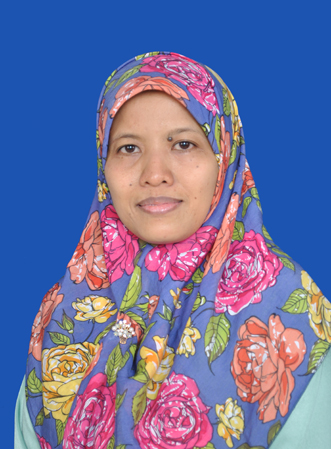
\includegraphics[height=0.2\textheight]{./ubah/Dini}
	\end{center}
%*********************************
\section*{Identity}
\begin{tabular}{p{3cm}cp{9cm}}
	%Masukan Identitas Disini.............
	Name  		  & :&
	Riandini \\
	Place of birth  & :&
		Jakarta\\
	Date of birth &:& 
		October $18^{th}$, 1977\\
	Address        &:& Depkes I, Jl. Husada I/79, Bekasi, 17412 \\
	%Identitas 1   &:&
	%	 Isi Identitas 1\\
	%Identitas 2   &:& 
	%	Isi Identitas 2\\
	%Identitas 3   &:&
	%	 Isi Identitas 3\\
	%Identitas 4   &:&
	%	 Isi Identitas 4\\
\end{tabular}

\section*{Education}
\begin{tabular}{p{3cm}cp{9cm}}
	2023-2027  	& :&
		Doctoral Degree (S3), Departement of Electrical Engineering, Faculty of Intelligent Electrical and Informatics Technology, Institut Teknologi Sepuluh Nopember\\
	&&\\
	2005-2007  & :&
		Master Degree (S2),Biomedical Engineering, University of Groningen\\
	&&\\
	1996-2001  & :&
		Bachelor Degree (S1), Department of Electrical Engineering, Institut Teknologi Bandung\\
	%&&\\
	%0000-0000  & :&
%		Pendidikan 1\\
	%&&\\
	%0000-0000  & :&
%		Pendidikan 2\\
%	&&\\
%	0000-0000  & :&
%		Pendidikan 3\\
\end{tabular}


\section*{Publications}

\begin{enumerate}
	\item Riandini, R., Purnama, K. E., Yuniarno, E. M., \& Purnomo, M. H. (2022, \large{bulan??}). Activation Function Selection for U-Net Multi-Structures Segmentation of End-Diastole and End-Systole Frames of Cine Cardiac MRI. In \textit{2022 IEEE Int. Conf. Imaging Systems and Techniques (IST)} (pp. ??). Taiwan (hybrid): IEEE.
	
	\item Riandini, Sardjono, T. A., Purnama, K. E., Yuniarno, E. M., \& Purnomo, M. H. (2023, June). A U-Net-Based System for Cine Cardiac Segmentation on MR Images: The Effect of Fuzzy Pooling Layer Type. In \textit{2023 IEEE Int. Symp. Medical Measurements and Applications (MeMeA)} \large{pp. ??}. Jeju, South Korea (hybrid): IEEE.
	
	\item Riandini, Yuniarno, E. M., Purnama, K. E., Aritsugi, M., \& Purnomo, M. H. (2025, July). Investigating Diverse Loss Functions for Myocardium Ring Segmentation in Cardiac Magnetic Resonance Images Using Fuzzy Pooling. \textit{Array}, 26, 100382, Elsevier. (Scopus Q1)
	
	\item Riandini, Setiadi, B., Yuniarno, E. M., Purnama, I. K. E., Aritsugi, M., \& Purnomo, M. H. (2026). MyoScarNet-RA: A Residual Attention Network for Myocardial Surface Area Quantification Based on Scar Segmentation. \textit{IEEE Access}, 14, 76722–76747. (Scopus Q1)
\end{enumerate}

\section*{Other Achievements and Research Experiences}
\begin{enumerate}
	\item International Grant from IEEE Engineering Projects in Community Service (EPICS), 2022, for the project titled: \textit{"\large{??}"}.
	\item National Book Chapter: \textit{Inovasi Teknologi Berbasis Kecerdasan Buatan dalam Bidang Kesehatan}. ISBN: 978-623-0275-84-5. Published in 2023 by Institut Teknologi Sepuluh Nopember, in collaboration with IEEE Industrial Electronics Society (IES) Indonesian Section and Deepublish.
	\item National Grant from Institut Teknologi Sepuluh Nopember (ITS), on the scheme of \textit{"\large{??}"}, 2025, for the research titled: \textit{"\large{??}"}.
	\item National Grant from Institut Teknologi Sepuluh Nopember (ITS), on the scheme of \textit{"\large{??}"}, 2025-2026, for the research titled: \textit{"\large{??}"}.
	\item Speaker in Webinar IEEE Industrial Application Society (IAS) - Indonesia Chapter, for the presentation titled: \textit{"AI dalam Kesehatan Jantung (Dari Diagnosis hingga Prediksi Risiko Penyakit)"}, July  $18^{th}$, 2026, 
\end{enumerate}

\cleardoublepage}
\newcommand{\DaftarPustaka}{\renewcommand{\bibname}{REFERENCES}
\addcontentsline{toc}{chapter}{\bibname}
\titlespacing*{\chapter}{0pt}{0ex}{5ex}
\appendix

%\bibliographystyle{IEEEtran}
%\bibliographystyle{harvard}
\bibliographystyle{plainnat}
\bibliography{IEEEabrv,./ubah/pustaka_dini}
\cleardoublepage}

\tolerance=9999
\emergencystretch=10pt
\hyphenpenalty=10000
\exhyphenpenalty=100